\chapter{Methodology}\label{ch:methodology}

\section{Methodology}\label{sec:methodology}

\subsection{Overall Research Approach}\label{sec:method-approach}

The four component studies adopt a Design Science Research (DSR) approach. This
method suits computer-science projects whose goal is to build something new and
demonstrate that it works: instead of studying a problem only in theory, the
researchers build a real, working system and test it. The DSR cycle used
throughout the project has four steps. First, understand the problem through the
literature review, which shows that no current system combines guarded intent
recognition, grounded planning, autonomous error recovery, and local
vulnerability analysis. Second, build the artefact: each component is
implemented as a working service with a defined interface contract. Third, test
the artefact on purpose-built data sets and measure the relevant quality
attributes. Fourth, report the design choices, the results, and the findings.

A controlled design-and-evaluation protocol was committed in advance. Each
component fixed its data-set construction, its evaluation measures, and its
comparison configurations before reporting results, and each component exposes
its committed artefacts (prediction files, test logs, and configuration) so that
the reported figures can be audited.

\subsection{Framework Architecture and Requirements}\label{sec:method-arch}

NeuroShell is organised as a four-component chain. \cref{fig:arch-ire} positions
the IRE within the stack; the identical chain is described in each component
report.

\begin{figure}[htbp]
  \centering
  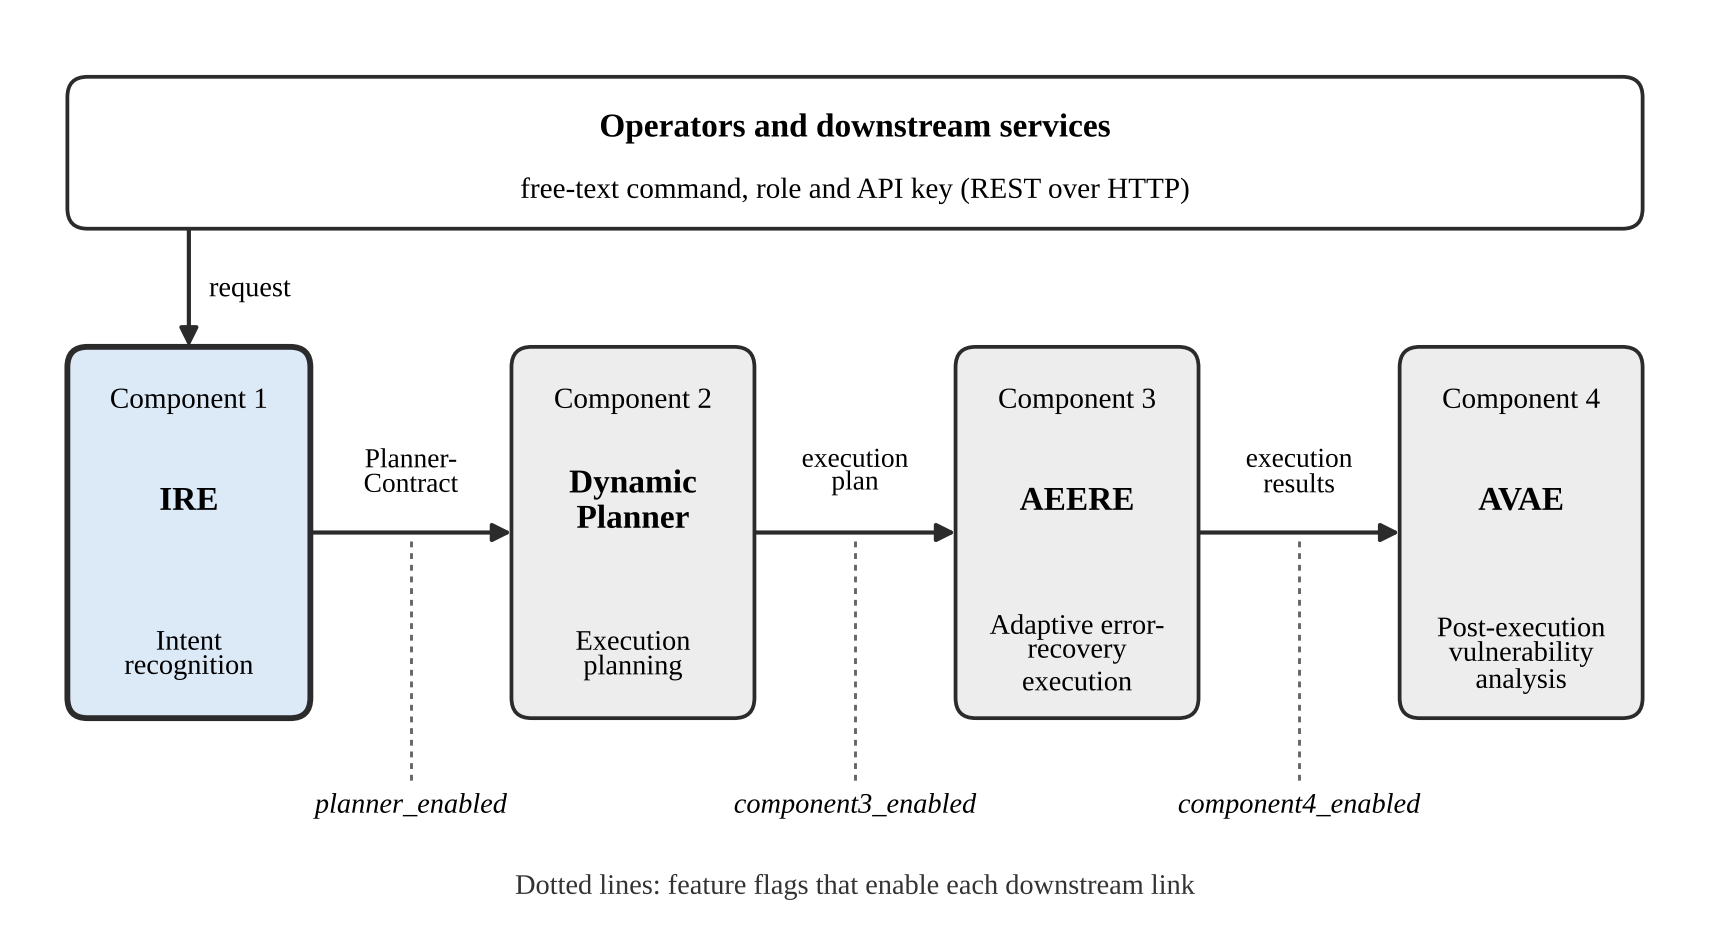
\includegraphics[width=0.9\textwidth]{C-01-Intetrecodnition Engine.pdf/vertopal_433ccb30063e47f1ba4c32a79683aeea/media/image6.png}
  \caption{Position of the Intent Recognition Engine within the NeuroShell
  four-component stack.}\label{fig:arch-ire}
\end{figure}

Each component is an independent FastAPI service that shares state through
Redis and communicates through structured JSON over HTTP. The IRE exposes the
entry point (port 8001) accepting natural language; the planner (port 8002)
accepts the intent contract and returns a validated command; the AEERE (port
8003) executes commands in a Docker sandbox and returns execution records; the
AVAE (port 8004) accepts execution records and returns structured, prioritised
vulnerability findings. \cref{tab:chain} summarises the four parts.

\begin{table}[htbp]
  \centering
  \begin{tabular}{@{}p{0.28\textwidth}p{0.68\textwidth}@{}}
    \toprule
    \textbf{Component} & \textbf{Job}\\
    \midrule
    C1 --- Intent Recognition Engine & Reads the plain-English request and
    turns it into structured JSON with the intent and details (port 8001).\\
    C2 --- Dynamic Planner \& RAG Engine & Turns the intent into a command by
    reading a store of tool documentation (port 8002).\\
    C3 --- Adaptive Execution \& Error-Recovery Engine & Runs the command in a
    sandbox, records the output and errors, and fixes failures on its own (port 8003).\\
    C4 --- AI-Driven Vulnerability Analysis Engine & Takes the logs from C3,
    finds weaknesses, and predicts how risky they are (port 8004).\\
    \bottomrule
  \end{tabular}
  \caption{The four parts of NeuroShell and their responsibilities.}\label{tab:chain}
\end{table}

\subsection{Methodology of the Intent Recognition Engine}\label{sec:method-ire}

The IRE methodology is a controlled design-and-evaluation study under a
committed protocol. The data set is a purpose-built, annotated collection of
1,500 security prompts: 600 well-formed records and 900 deliberately flawed
records spanning eight flaw classes (adversarial utterances, RBAC violations,
fabricated parameters, type mismatches, fabricated CVEs, contradictory
requests, out-of-scope targets, and ambiguous requests). Every record carries a
committed ground-truth label so that per-record decisions can be scored
deterministically.

The artefact is a seven-stage pipeline wrapped in five middleware components
(see \cref{fig:ire-pipeline}): the raw output of an offline language model is
parsed into a proposition, then validated for structure, target syntax, and
authorisation before an intent contract is emitted. Middleware adds the
authorisation checks, an adversarial-utterance detector, and a
hallucination-validation gate that enforces the safety invariant that every
accepted intent is schema-valid, authorised, and in scope.

\begin{figure}[htbp]
  \centering
  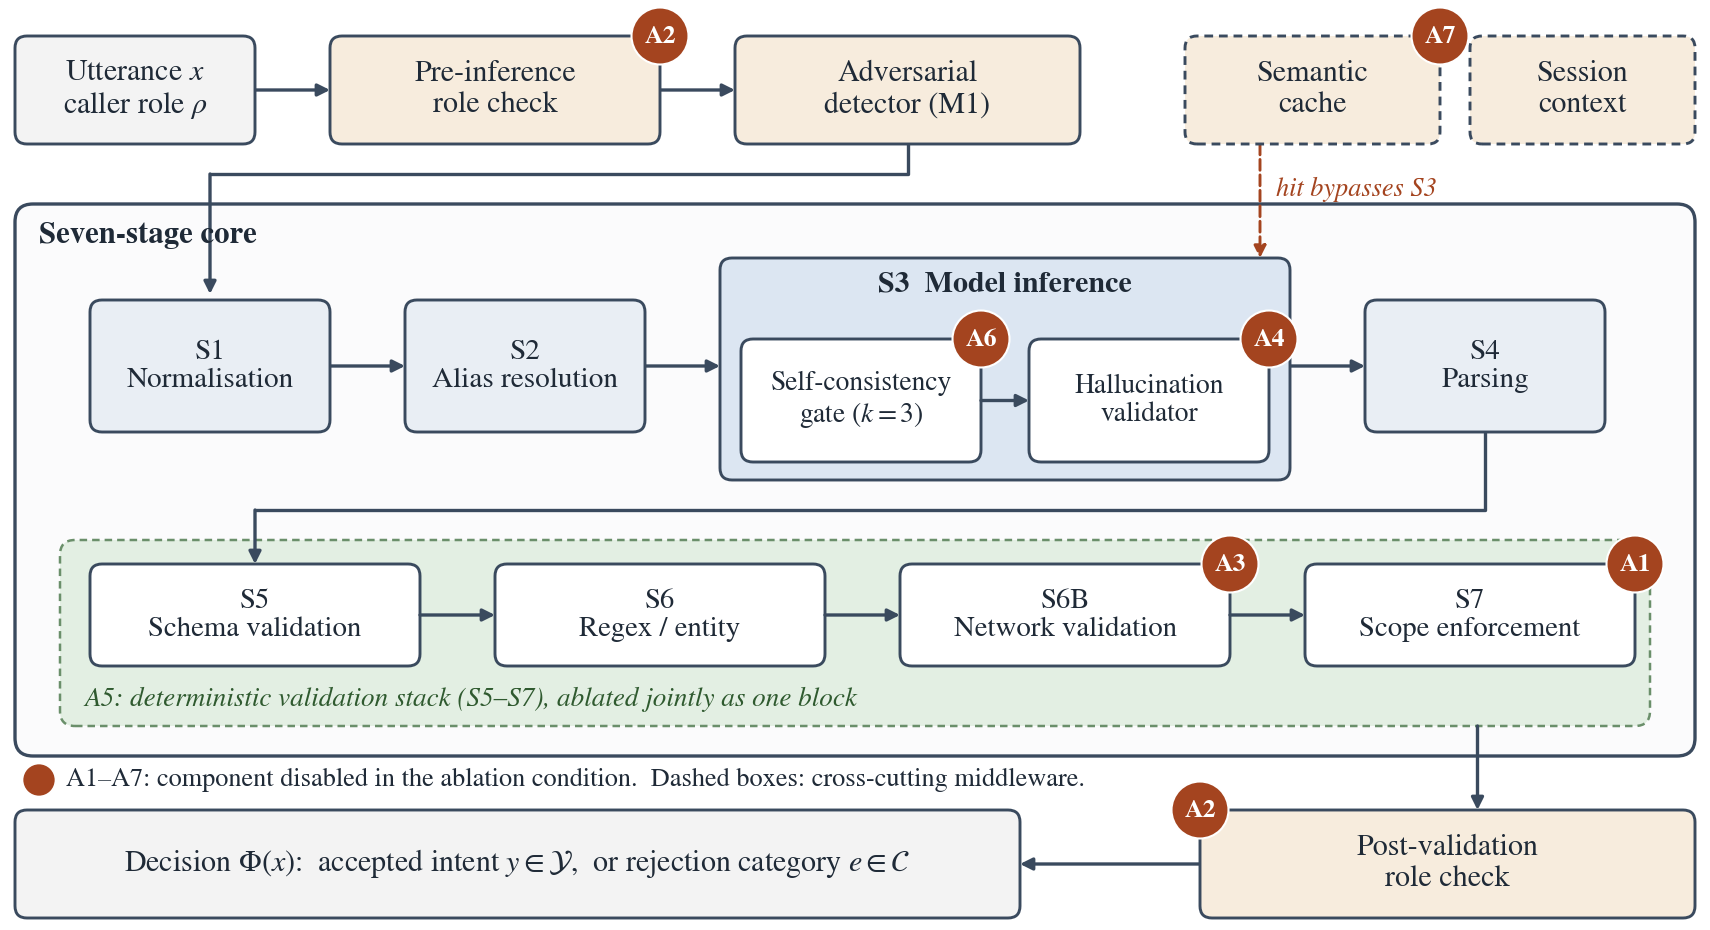
\includegraphics[width=0.9\textwidth]{C-01-Intetrecodnition Engine.pdf/vertopal_433ccb30063e47f1ba4c32a79683aeea/media/image4.png}
  \caption{The guarded pipeline of the IRE and the ablation protocol used to
  quantify the contribution of each layer.}\label{fig:ire-pipeline}
\end{figure}

Four experiments are defined. Experiment~1 measures the value of the whole
pipeline against raw model output. Experiment~2 compares two offline backends
(Gemma and Qwen) under an identical guardrail stack. Experiment~3 performs a
per-layer ablation in which one protection is removed at a time to quantify each
layer's contribution to safety. Experiment~4 reports the catch rate for each
flaw class separately. All results are single-run point estimates obtained on
one CPU-only machine, which limits cross-platform generalisation.

\subsection{IRE Architecture and Requirements}\label{sec:method-ire-req}

The IRE is a modular Python service with a FastAPI interface, running as a local
daemon under the Uvicorn ASGI server on port 8001. Its source tree comprises ten
packages under \emph{src/} (among them \emph{api}, \emph{integration},
\emph{middleware}, \emph{pipeline}, and \emph{validation}), with central
configuration in \emph{config/}. Role-based access control (RBAC), enforcement
and feature policies are held in separate Python modules and a YAML file, and
runtime constants are loaded from the environment and the YAML flags at start-up,
so that every experimental constant is reproducible from the committed
configuration. A health start-up gate checks the environment file, Ollama
connectivity (port 11434) and model availability before serving.

The requirements were specified against the IEEE 830 recommended practice for
software requirements specifications. \cref{tab:ire-fr} lists the functional
requirements of the IRE grouped under four product functions, each with the
component that realises it, and \cref{tab:ire-nfr} states the non-functional
requirements with the design provision that satisfies each one. The functional
requirements establish a direct trace from ``what the component must do'' to the
pipeline stage or middleware that implements it, which is the basis for the
verification gate described later.

\begin{table}[htbp]
  \centering
  \begin{tabular}{@{}p{0.14\textwidth}p{0.07\textwidth}p{0.45\textwidth}p{0.20\textwidth}@{}}
    \toprule
    \textbf{Group} & \textbf{ID} & \textbf{Requirement} & \textbf{Realised by}\\
    \midrule
    Core understanding & FR-1 & Normalise the input utterance. & S1 Input Normaliser\\
    & FR-2 & Resolve offensive-security aliases (for example \emph{EternalBlue} to CVE-2017-0144) to canonical identifiers. & S2 Alias Resolver\\
    & FR-3 & Classify the request into one of nine top-level intents. & S3 inference; S5 schema validation\\
    & FR-4 & Refine the intent into a hierarchical sub-intent that drives downstream tool selection. & Sub-intent classifier; Contract Builder\\
    Safety and security & FR-5 & Detect adversarial input before inference. & M1 Adversarial Detector\\
    & FR-6 & Enforce role-based access control both before and after inference. & M2 and M5 RBAC Guard\\
    & FR-7 & Validate model output against typed-schema, regular-expression, network and engagement-scope rules. & S5, S6, S6B and S7\\
    & FR-8 & Classify every failed validation into one of six hallucination classes. & Enforcement policy\\
    & FR-9 & Emit an audit record for every parse. & Audit logger\\
    Intelligence and quality & FR-10 & Maintain per-session context across turns. & M3 Session Context\\
    & FR-11 & Serve identical intents from a semantic cache. & M4 Semantic Cache\\
    & FR-12 & Gate low-confidence decisions through a self-consistency stage. & Self-consistency stage\\
    & FR-13 & Provide an optional XAI attribution path (disabled by default). & Feature flag only\\
    System and integration & FR-14 & Expose a REST API for parsing, execution and administration. & REST API\\
    & FR-15 & Push validated contracts to downstream components on a feature-flagged basis. & Contract Builder\\
    & FR-16 & Persist an append-only audit trail. & Audit logger\\
    & FR-17 & Make every guard individually disable-able through configuration. & Feature-flag configuration\\
    \bottomrule
  \end{tabular}
  \caption{Functional requirements of the IRE and the stages/middleware that
  realise them (from the IEEE 830-based requirements specification).}\label{tab:ire-fr}
\end{table}

\begin{table}[htbp]
  \centering
  \begin{tabular}{@{}p{0.15\textwidth}p{0.45\textwidth}p{0.29\textwidth}@{}}
    \toprule
    \textbf{Attribute} & \textbf{Requirement} & \textbf{Design provision}\\
    \midrule
    Performance & Adversarial detection completes in low milliseconds; RBAC fast-fail runs before any model cost; cache hits short-circuit the pipeline. & Lightweight lexical and structural scoring in M1; M2 placed ahead of S3; M4 bypasses inference on a hit.\\
    Reliability & Failure in non-critical middleware (session context, cache, adversarial detection) degrades gracefully and does not abort the request. & S7 independently re-scans the raw input for injection, so losing M1 does not remove all injection screening.\\
    Security & The service holds no credentials beyond an operator API key; rate limiting protects the model backend; no free-form model output is ever returned. & Local daemon with a single shared API key; only schema-validated contracts leave the engine (S4 to S7).\\
    Operability & Every stage and middleware is configurable through feature flags; the model family and engagement scope are reconfigurable at runtime; evaluation is reproducible from a single manifest. & Administrative views for feature flags, models and engagement scope; an evaluation manifest that pins the sampling configuration.\\
    \bottomrule
  \end{tabular}
  \caption{Non-functional requirements of the IRE and the design provisions.}\label{tab:ire-nfr}
\end{table}

\subsection{IRE Detailed Design: Stages, Middleware and Enforcement}\label{sec:method-ire-design}

The IRE pipeline is organised as seven core stages wrapped in five middleware
components. Stages S1--S4 prepare the input and the model output. S1 normalises
casing, whitespace and Unicode (NFKC form) and standardises jargon terms into
canonical phrases. S2 resolves aliases, such as \emph{nmap -sS} to a SCAN action
and exploit names to canonical CVE identifiers, using the alias map in
\emph{data/alias\_map.json}. S3 instructs the model to emit a fixed JSON schema
at the sampling configuration pinned in the evaluation manifest. S4 recovers the
JSON payload by stripping code fences, markdown artefacts and thinking tags.

The remaining stages are deterministic validators, shown in
\cref{tab:ire-validators}. Because S5--S7 recompute every check without further
model calls, a model output can be exposed only if it satisfies all of them; the
deterministic guard path is therefore bit-exact and auditable, which is a
reproducibility property that the evaluation protocol relies on.

\begin{table}[htbp]
  \centering
  \begin{tabular}{@{}p{0.26\textwidth}p{0.69\textwidth}@{}}
    \toprule
    \textbf{Stage} & \textbf{Checks performed}\\
    \midrule
    S5 Schema Validator & Exactly one of nine \emph{IntentType} values; a matched target type; ports in the range 1--65535; CVE syntax \emph{CVE-YYYY-NNNN}; confidence in {[}0,1{]}; \emph{AMBIGUOUS} requires confidence below 0.5; \emph{REJECTED} requires a rejection reason.\\
    S6 Regex Validator & Deterministic re-verification of every entity produced by the model (IPv4 and IPv6 addresses, CIDR blocks, CVE identifiers, ports and URLs) and the absence of shell metacharacters.\\
    S6B Network Validator & Targets fall inside the configured engagement CIDR (default 192.168.0.0/16); permitted scan prefix lengths range from /30 (widest) to /32 (narrowest); target type is consistent with target value.\\
    S7 Scope Guard & Rejects out-of-scope targets in strict mode, warns in research mode; applies RFC 1918 private-address membership; re-scans the raw input as an injection gate.\\
    \bottomrule
  \end{tabular}
  \caption{Deterministic checks performed by the validation stages S5 to S7
  including S6B.}\label{tab:ire-validators}
\end{table}

The middleware provides the safety and quality functions around the core.
\cref{tab:ire-middleware} summarises the responsibilities of each middleware
component. The adversarial detector (M1) is a three-layer scorer: a lexical
layer scores known injection phrases and control tokens (weights 0.8--1.0), a
structural layer scores encoded payloads, script-like constructs and
imperative-but-unclassifiable phrasing (weights 0.3--0.9), and a scoring layer
fuses the signals into a cumulative score. A score at or above 0.7 flags the
request for downstream treatment and a score at or above 0.95 blocks it
immediately, before inference. Two-phase RBAC (M2 pre-inference, M5
post-inference) prevents a single bypassed guard from manufacturing an
authorised action; unknown roles are coerced to \emph{viewer}, the
least-privileged class. Session context (M3) maintains per-session turn history
with a time-to-live and injects the recent memory window into the prompt so that
anaphoric follow-ups such as ``the same target'' resolve correctly. The semantic
cache (M4) combines an exact hash with embedding similarity (sentence-transformers
\emph{all-MiniLM-L6-v2}) and short-circuits the LLM on a hit, pruning latency and
improving determinism; cache entries are invalidated together with the offline
CVE-grounding index so that cached decisions do not outlive the data they depend
on.

\begin{table}[htbp]
  \centering
  \begin{tabular}{@{}p{0.26\textwidth}p{0.68\textwidth}@{}}
    \toprule
    \textbf{Middleware} & \textbf{Responsibility}\\
    \midrule
    M1 Adversarial Detector & Three-layer lexical/structural/scoring gate before inference; flags at \(\ge0.7\), auto-blocks at \(\ge0.95\).\\
    M2 + M5 RBAC Guard & Two-phase authorisation around the core; unknown roles coerced to \emph{viewer}.\\
    M3 Session Context & Per-session turn history with TTL; memory window injected into the prompt.\\
    M4 Semantic Cache & Exact-hash plus embedding similarity; LRU-style eviction; invalidated with the CVE index.\\
    \bottomrule
  \end{tabular}
  \caption{The middleware components of the IRE and their responsibilities.}\label{tab:ire-middleware}
\end{table}

Every failed validation is classified into one of six hallucination classes and
recorded as an audit-grade \emph{ValidationFinding}. The enforcement policy maps
each class to one of three outcomes, BLOCK, WARN or ESCALATE
(\cref{tab:ire-hallucination}). Fabricated parameters, contradictory
action--target pairings, target-type mismatches and malformed fabricated CVEs
hard-block; ungrounded confidence (a syntactically valid but unindexed CVE)
warns; and out-of-scope targets warn in research mode but block in strict
production mode. Escalations are routed through an administrative escalation
queue for explicit human approval. This taxonomy is what lets the evaluation
report per-flaw-class catch rates rather than a single opaque rejection count.

\begin{table}[htbp]
  \centering
  \begin{tabular}{@{}p{0.28\textwidth}p{0.44\textwidth}p{0.19\textwidth}@{}}
    \toprule
    \textbf{Hallucination class} & \textbf{Description} & \textbf{Outcome}\\
    \midrule
    Fabricated parameters & Parameter values invented by the model. & BLOCK\\
    Contradictory action--target pairing & An action incompatible with the stated target. & BLOCK\\
    Target-type mismatch & A target value inconsistent with its declared type. & BLOCK\\
    Malformed fabricated CVE & An invented identifier that fails CVE syntax. & BLOCK\\
    Ungrounded confidence & A syntactically valid CVE absent from the offline index. & WARN\\
    Out-of-scope target & A target outside the declared engagement scope. & WARN in research; BLOCK in strict\\
    \bottomrule
  \end{tabular}
  \caption{Hallucination classes and their enforcement outcomes.}\label{tab:ire-hallucination}
\end{table}

\subsection{IRE Design Decisions}\label{sec:method-ire-decisions}

Seven principal design decisions shaped the IRE; each is recorded as a choice
between a credible alternative and the adopted design
(\cref{tab:ire-decisions}). Three of these decisions recur at framework level.
First, the decoder is local and CPU-only because a cloud-hosted model would
contradict the closed trust boundary. Second, output is a fixed validated JSON
schema rather than free-form prose, converting a plausibility claim into a
verifiable one. Third, validation is deterministic rather than model self-checked,
avoiding drift and reusing the same fallible estimator that produced the output.
The IRE additionally chooses \emph{no retrieval at inference time}: retrieved
text is itself a prompt-injection vector, so offline CVE grounding is loaded at
start-up only, keeping the threat model closed.

\begin{table}[htbp]
  \centering
  \begin{tabular}{@{}p{0.15\textwidth}p{0.25\textwidth}p{0.24\textwidth}p{0.25\textwidth}@{}}
    \toprule
    \textbf{Decision area} & \textbf{Alternative considered} & \textbf{Adopted design} & \textbf{Principal rationale}\\
    \midrule
    Decoder & Cloud-hosted model & Local model through Ollama, CPU-only & No request leaves the device; no credentials held\\
    Output form & Free-form prose & Fixed JSON schema validated by S4--S7 & Converts a plausibility claim into a verifiable one\\
    Validation & Model self-checking & Deterministic rules (S5--S7, S6B) & Avoids drift; bit-exact and auditable\\
    Grounding & Retrieval-augmented generation & No retrieval at inference time & Removes the retrieved-text injection vector\\
    Access control & Single post-hoc RBAC check & Two-phase RBAC (M2 and M5) & A bypassed guard cannot yield an authorised action\\
    Confidence & Single-pass model confidence & Self-consistency gate for low-confidence decisions & Calibrated scores are unreliable for small offline models\\
    Latency & Inference on every request & Two-channel semantic cache (M4) & Short-circuits repeated intents; improves determinism\\
    \bottomrule
  \end{tabular}
  \caption{The seven principal design decisions of the IRE.}\label{tab:ire-decisions}
\end{table}

The planner methodology follows the same DSR pattern with an explicit
experimental protocol. The planning workflow is organised into distinct stages:
intent interpretation, documentation retrieval, tool selection, command
synthesis, and validation. This separation makes the responsibility of each
stage explicit and allows the component to be developed and tested through
structured inputs without requiring the complete framework to be active for
every test.

The data set for the held-out assessment consists of 337 cases covering the
three supported tools (113 Nmap, 116 Nikto, and 108 Gobuster), each with a
reference command. Direct assessment compares the base and adapted
configurations on these held-out cases and reports strict exact-match rates by
tool. A separate 25-case experiment examines the base model with and without
retrieval, measuring semantic command accuracy, normalised exact-match rate,
tool-selection accuracy, and planning latency, isolating the effect of
documentation grounding. \cref{fig:planner-arch} shows the internal architecture
of the component.

\begin{figure}[htbp]
  \centering
  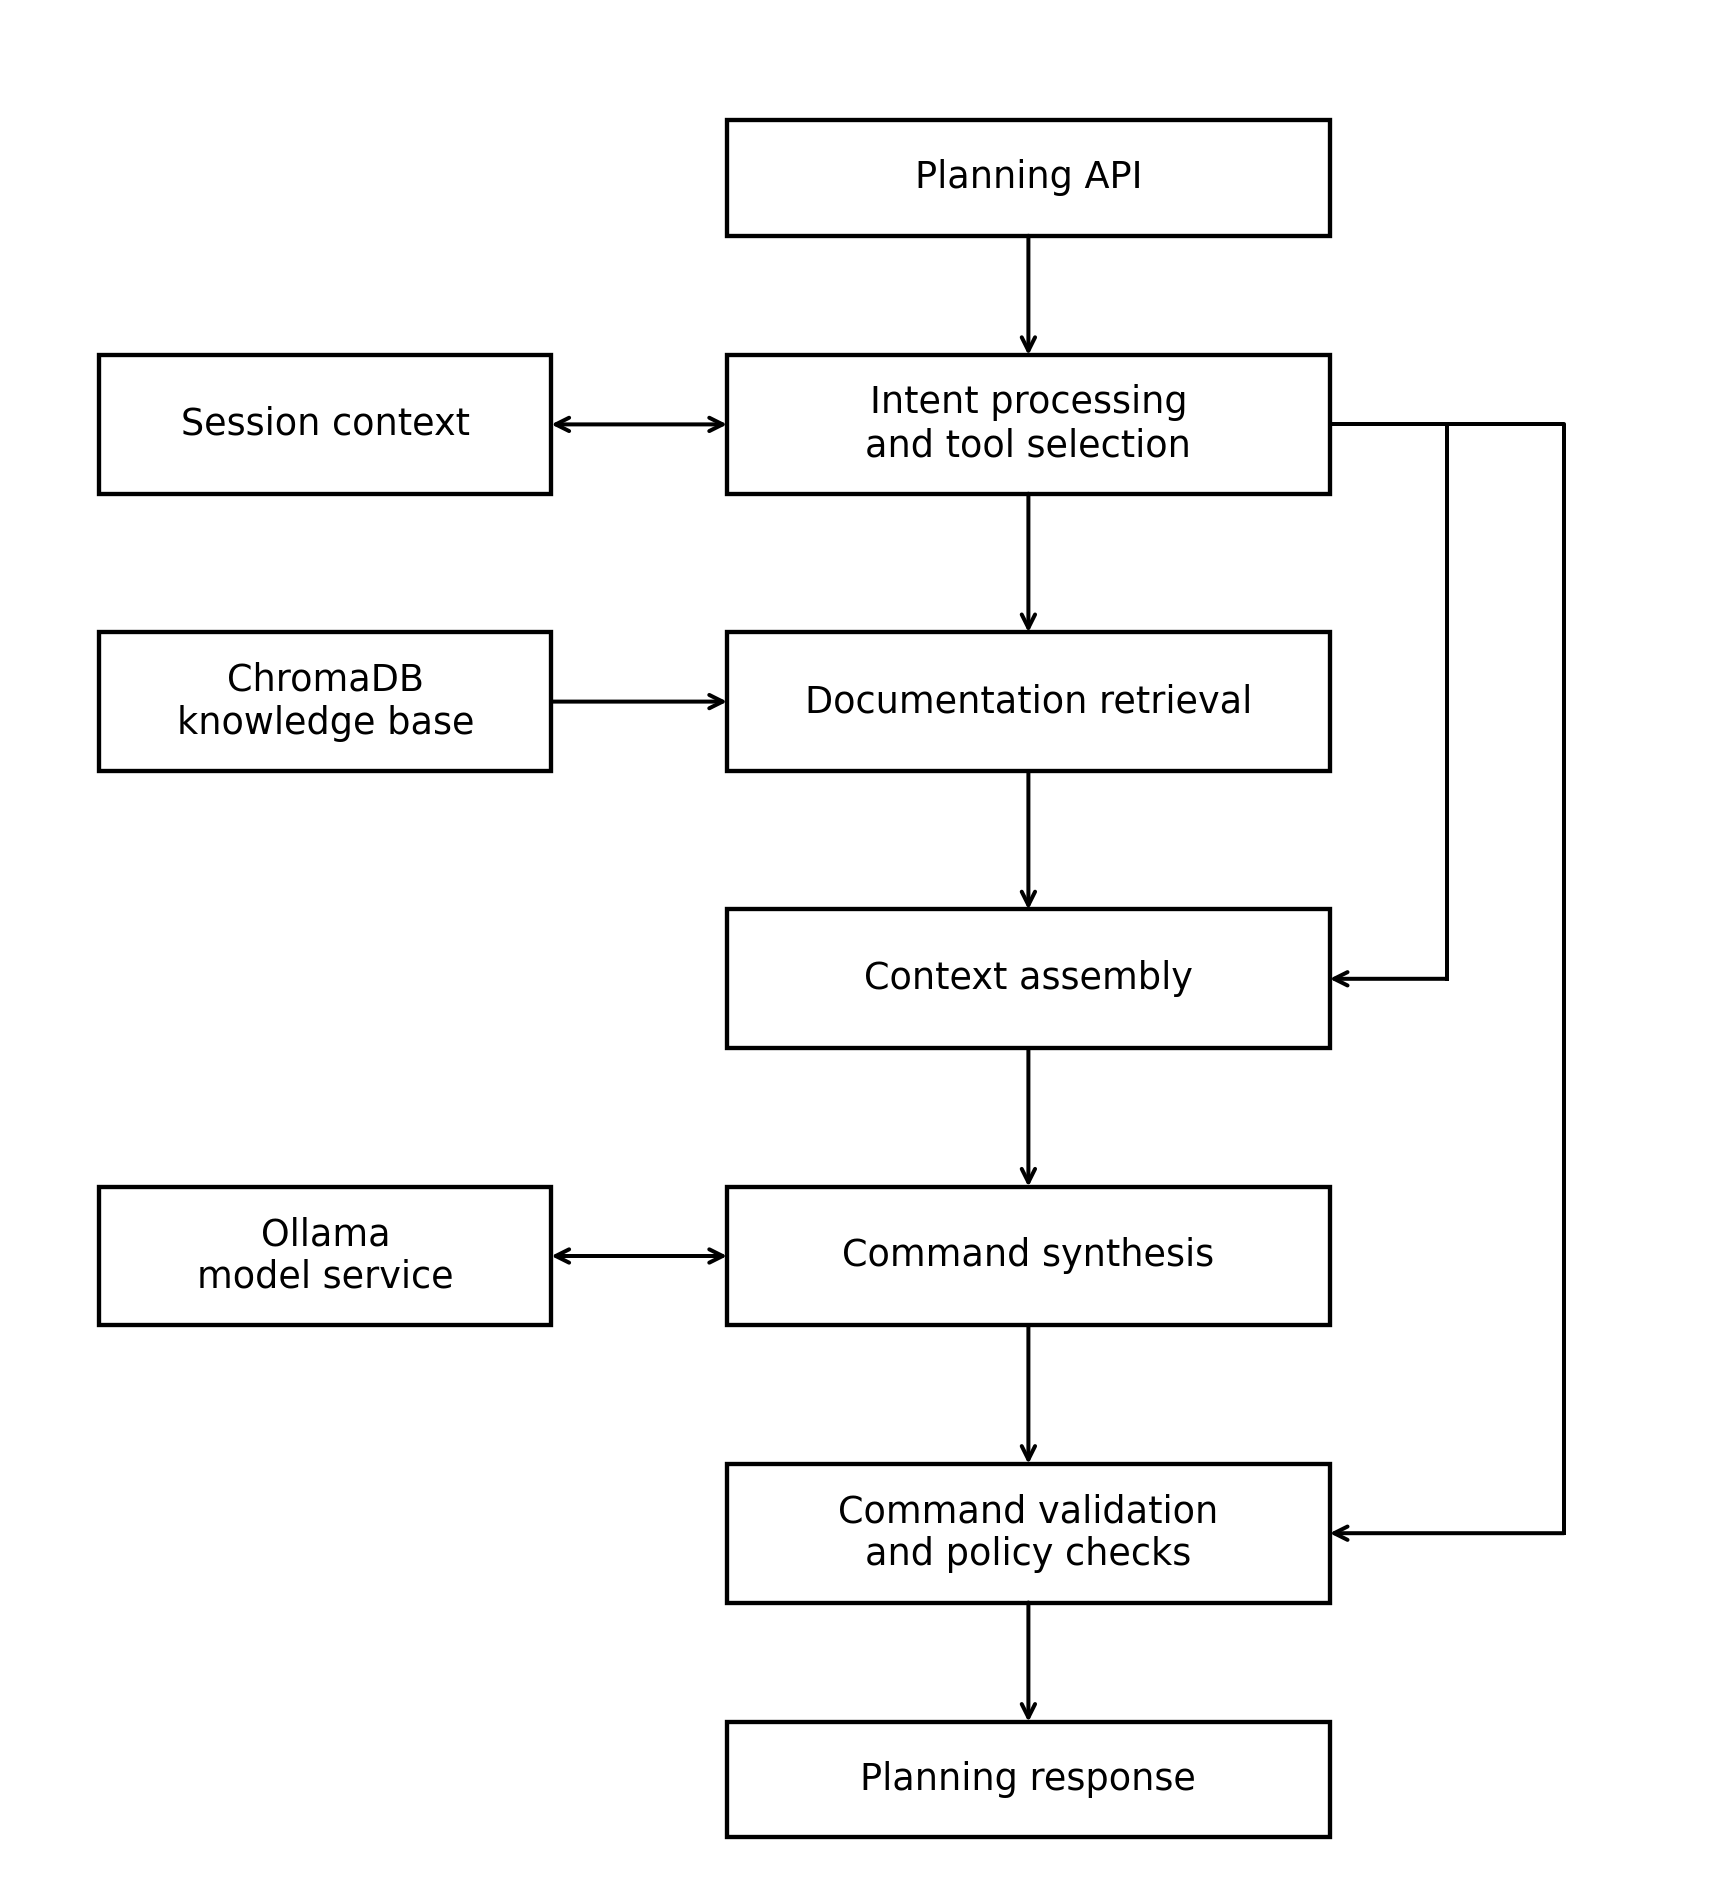
\includegraphics[width=0.85\textwidth]{C-02-Dynamic planner and rag enginee/vertopal_80eb40840323498cb949d017d9b2b63a/media/image2.png}
  \caption{Internal architecture of the Dynamic Planner and RAG Engine.}\label{fig:planner-arch}
\end{figure}

Measures and evaluation cover tool-selection accuracy, command syntax
correctness, semantic alignment, safety behaviour, and generation latency.
Rejection outcomes record whether the configured checks accept valid, in-scope
requests and reject invalid or out-of-policy requests. The knowledge base stores
documentation passages in ChromaDB with embeddings produced by
\emph{all-MiniLM-L6-v2}, and retrieval results are passed to the synthesising
model as context.

\subsection{Methodology of the Adaptive Execution and Error-Recovery Engine}\label{sec:method-aeere}

The AEERE was designed and tested using DSR. The engine works in five stages
that form a loop: run the command in a fresh Docker container running Kali
Linux; label the error; work out the cause; fix and check; and retry or stop
nicely. A fixed command returns to the run stage, and the cycle repeats until
the command works or the retry limit for that error type is reached. The engine
detects silent failures as well: a tool that exits with code 0 but produces no
useful output is treated as a failure (\cref{fig:aeere-loop}).

\begin{figure}[htbp]
  \centering
  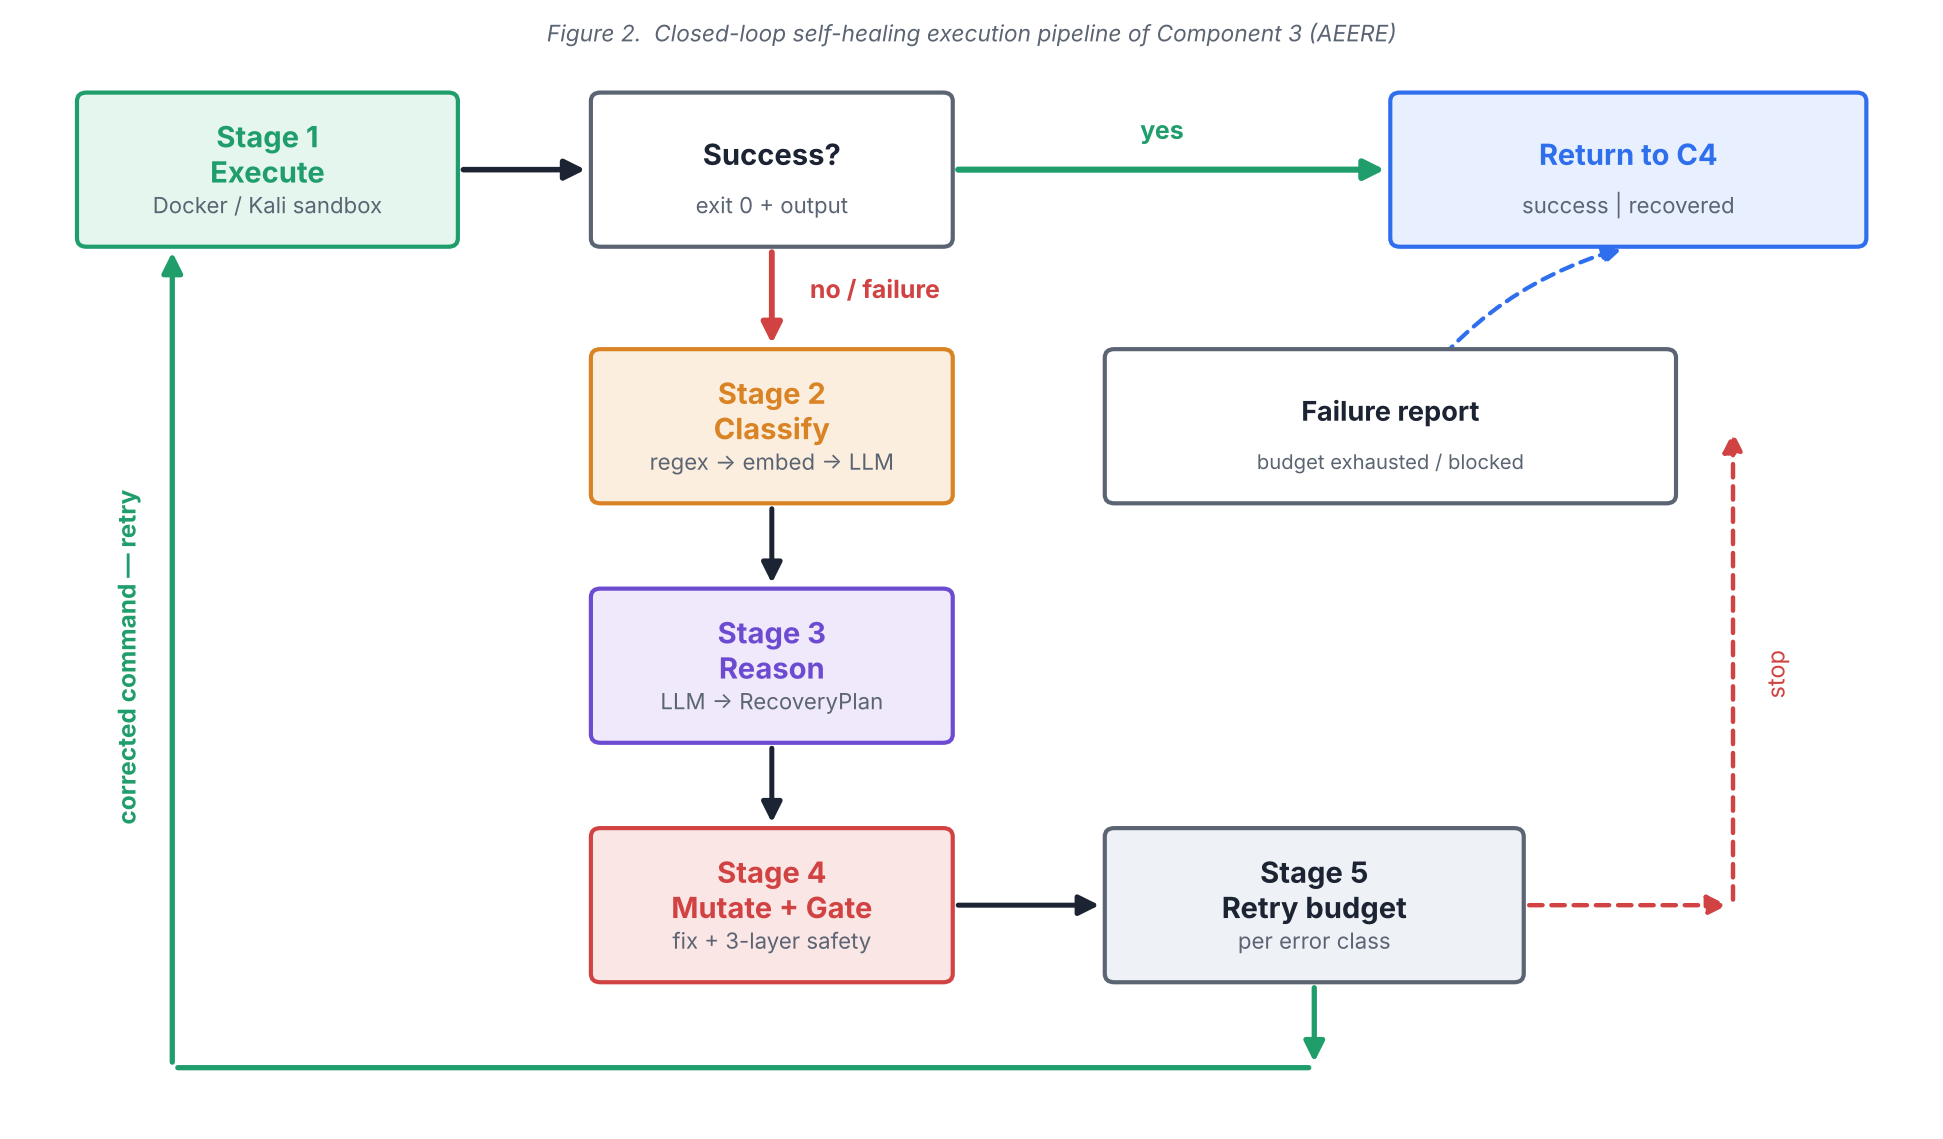
\includegraphics[width=0.9\textwidth]{C-03-Adoptive executer and error Recovery engine/vertopal_05e97fad080746c9b767567e93f99da6/media/image2.png}
  \caption{The five-stage error-recovery loop of the AEERE.}\label{fig:aeere-loop}
\end{figure}

Error labelling uses a three-step cascade that trades speed against thinking
power (\cref{fig:aeere-cascade}). Step 1 is a set of hand-written patterns tied
to an eight-type error list built specifically for Kali offensive-security tool
failures. Step 2 is a text-similarity check: a character n-gram TF-IDF vector
with logistic regression, trained only on the training half of the data set,
which accepts a match only above a 0.70 threshold. Step 3 is a local AI model
(Gemma run through Ollama) that receives the original command, the full error
message, the exit code, the possible error type, and task context, and replies
with a small JSON plan containing the cause, the chosen fix, and a corrected
command. The first step that labels the error stops the slower ones, so simple
errors stay cheap and fast.

\begin{figure}[htbp]
  \centering
  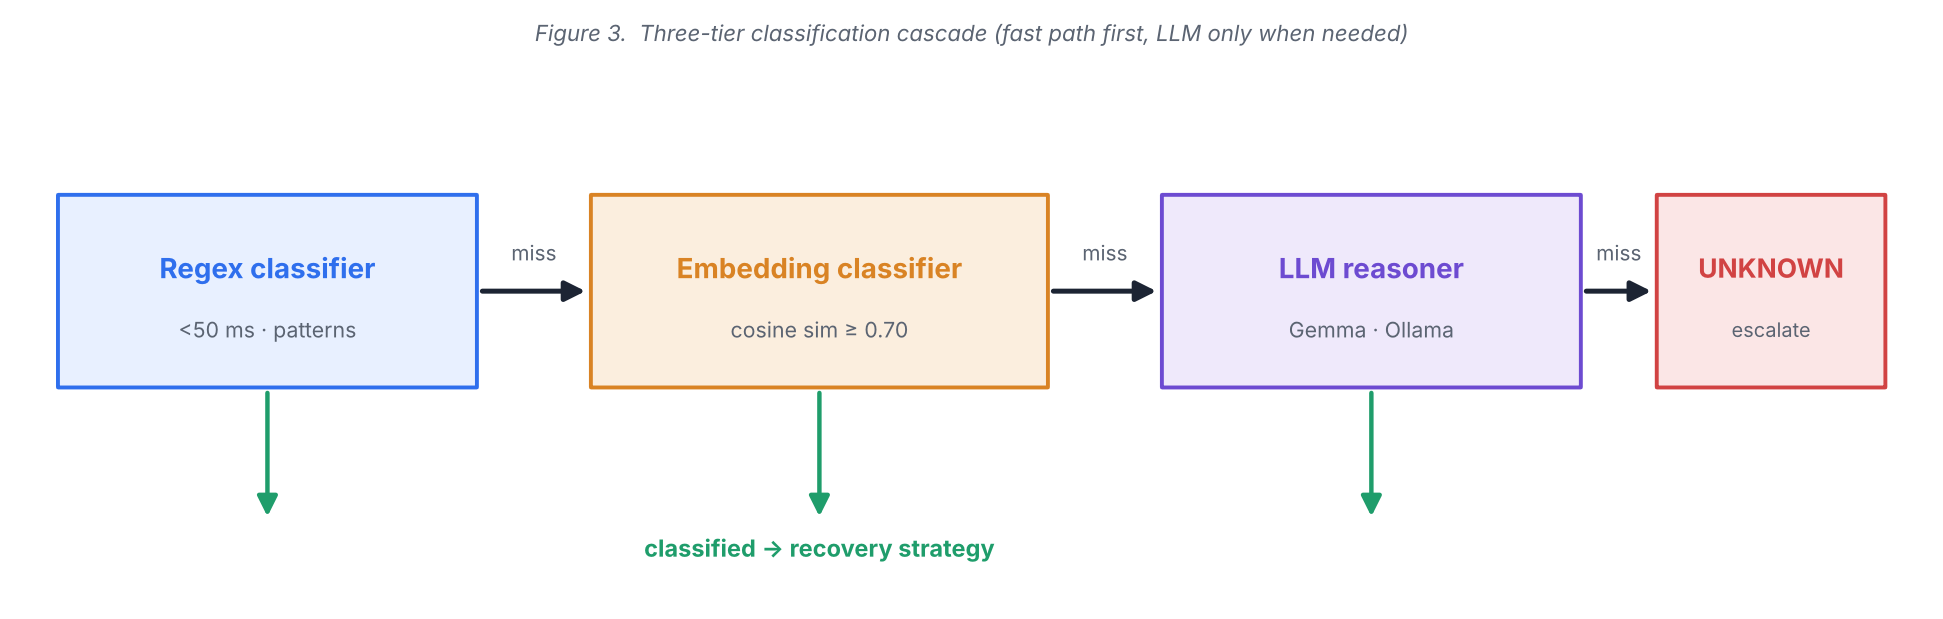
\includegraphics[width=0.9\textwidth]{C-03-Adoptive executer and error Recovery engine/vertopal_05e97fad080746c9b767567e93f99da6/media/image3.png}
  \caption{The three-step error check: fast path first; the AI is used only for
  new or unusual errors.}\label{fig:aeere-cascade}
\end{figure}

Every fixed command must pass three safety checks before it is allowed to run:
a format check on the AI's reply, a dangerous-word check that blocks destructive
or fetch-and-execute patterns (for example \texttt{rm -rf}, disk wiping, or
downloading and running code), and a confidence-and-scope check that requires a
minimum confidence level and rejects any target outside private RFC-1918 address
ranges. Every blocked case is written to a log in an SQLite database, which is
the evidence base for the safety tests.

The error list itself, shown in \cref{tab:aeere-errorlist}, is a contribution of
the work: it is the first of its kind for Kali offensive-security tool failures.
Each error type carries the example signs that point to it, the default fix, the
retry limit, and the wait rule. The engine also keeps a tool-swap list: when a
tool fails for good (its retry limit is used up), the engine swaps in a
different tool that does the same job, for example gobuster may be swapped for
ffuf or dirb for folder scanning, and nmap for masscan or rustscan for network
scanning, so the task can still finish.

\begin{table}[htbp]
  \centering
  \begin{tabular}{@{}p{0.18\textwidth}p{0.27\textwidth}p{0.27\textwidth}p{0.16\textwidth}@{}}
    \toprule
    \textbf{Error type} & \textbf{Example sign} & \textbf{Fix} & \textbf{Retries / wait}\\
    \midrule
    Tool not installed & command not found; exit 127 & Install with apt-get, then retry & 2 / fixed\\
    Permission denied & Permission denied; EACCES & Add sudo & 2 / fixed\\
    Network unreachable & No route to host; refused & Change timing / settings & 3 / growing\\
    Wrong syntax & Invalid option; usage: & Rewrite the flags & 2 / fixed\\
    Out of resources & Cannot allocate memory; ENOMEM & Lower threads / load & 2 / fixed\\
    Login failure & Authentication failed; publickey & Try another login method & 2 / fixed\\
    Timeout & ETIMEDOUT; timed out & Raise timeout / reduce scope & 3 / growing\\
    Version mismatch & deprecated; unknown option & Rewrite for the installed version & 1 / fixed\\
    \bottomrule
  \end{tabular}
  \caption{The eight error types of the AEERE error list and how each is
  fixed.}\label{tab:aeere-errorlist}
\end{table}

Building the test data set was a contribution in itself. There was no
ready-made public data set of Kali tool failures with correct fixes labelled,
so one was built: after planning for a minimum of 80 cases (at least ten per
error type), it was grown to 8,000 labelled command-failure cases. Each case
records the command, the raw error message, the exit code, the correct error
type, the cause, and the best fix. The data set covers ten error types, more
than eighteen tools (including netcat, gobuster, sqlmap, hashcat, nikto, ssh,
nmap, docker, dirsearch, and john), and three difficulty levels (2,663
beginner, 2,632 intermediate, and 2,705 advanced cases). All addresses in the
cases are private RFC-1918 lab addresses. \cref{fig:aeere-dataset} shows the
distribution across error types.

\begin{figure}[htbp]
  \centering
  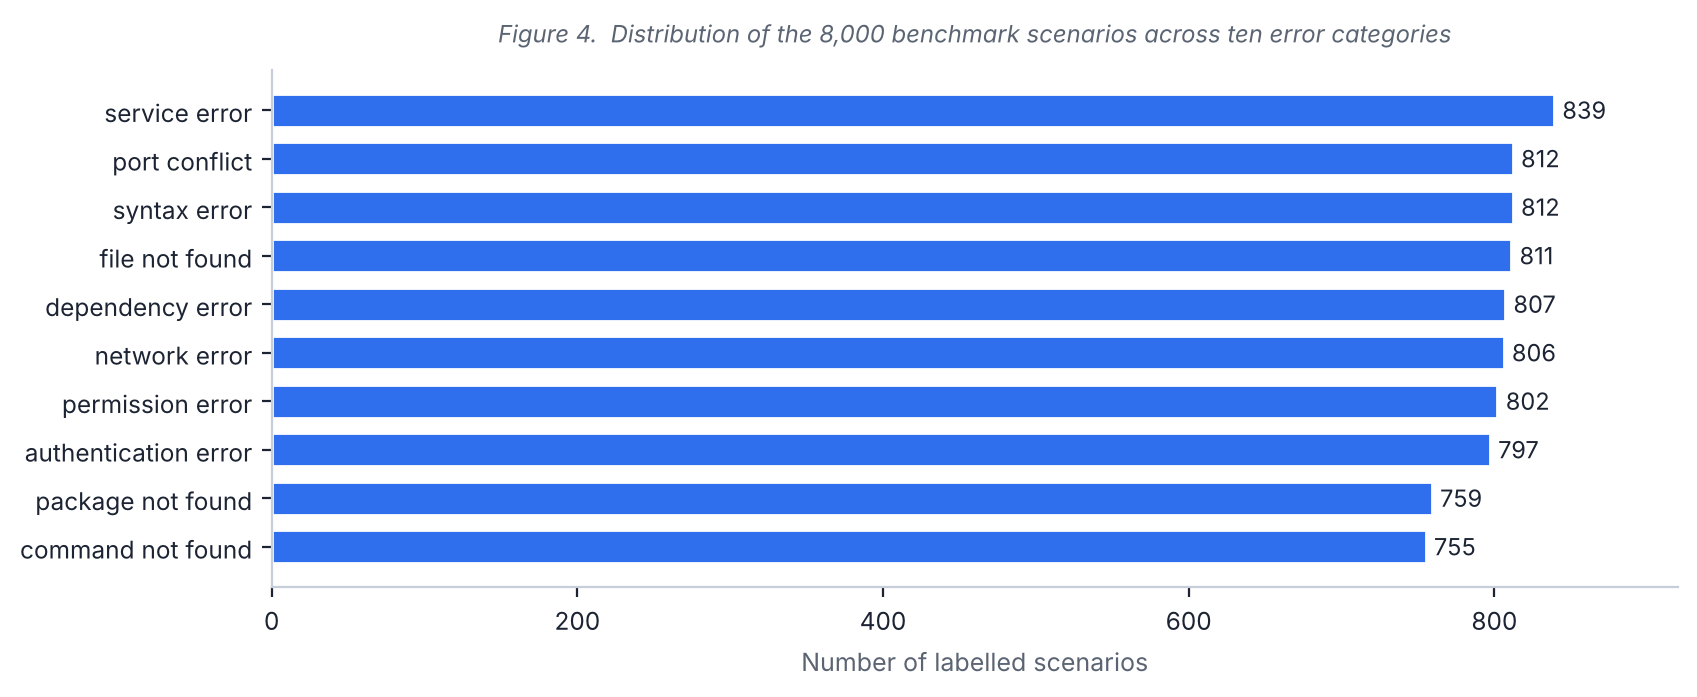
\includegraphics[width=0.9\textwidth]{C-03-Adoptive executer and error Recovery engine/vertopal_05e97fad080746c9b767567e93f99da6/media/image4.png}
  \caption{The 8,000 test cases spread across ten error types.}\label{fig:aeere-dataset}
\end{figure}

The error-labelling test was run in Python with scikit-learn. The 8,000 cases
were split into a training set (70\%, 5,600 cases) and a test set (30\%, 2,400
cases). The split was stratified so that every error type keeps the same share
in both halves, and a fixed random seed was used so the result can be repeated.
A second, harder test added controlled noise to each test message (log prefixes
and timestamps, trailing text, changed case, keyboard-style typos, and
truncation) with the noise level raised step by step from 0\% to 60\%, while the
text model remained trained only on the clean training half.

\subsection{Methodology of the AI-Driven Vulnerability Analysis Engine}\label{sec:method-avae}

The AVAE methodology combines vulnerability data preparation, feature
engineering, machine-learning model training, performance evaluation, and
component implementation. The primary data set is a curated collection of
155,852 vulnerability records derived from public vulnerability sources,
containing severity information, exploitation-related indicators, publication
details, and CISA KEV membership information. The NVD, CISA KEV catalogue, and
EPSS provide supporting intelligence. After cleaning (removing duplicates,
handling invalid values, converting attributes to numerical formats, and
computing vulnerability age from publication dates), the data set supported
154,889 class-0 records (no recorded KEV membership) and 963 class-1 records
(recorded KEV membership).

Feature selection produces five numerical features: CVSS v3 score, EPSS score,
EPSS percentile, vulnerability age, and an engineered interaction feature
computed as the product of the CVSS v3 score and the EPSS score. The
classification target is binary and derived from CISA KEV membership. XGBoost
was selected because it supports nonlinear relationships and efficient learning
from structured numerical data; hyperparameter tuning examined the number of
estimators, maximum tree depth, learning rate, minimum child weight, and
training-weight configuration, with validation performance (and specifically
PR-AUC) used to support model selection. SHAP was incorporated to describe the
contribution of individual features to the model's output, for both local
explanations of individual predictions and global feature-importance analysis.
Evaluation uses accuracy, precision, recall, F1-score, ROC-AUC, and PR-AUC,
together with a confusion matrix for error analysis.

The implemented component combines scanner-output parsing (Nmap, Nikto, and
Gobuster), vulnerability-intelligence enrichment, the trained classifier, SHAP
explanations, contextual risk prioritisation, Neo4j graph persistence, and a
FastAPI interface. \cref{fig:avae-shap} illustrates the feature-engineering
implementation used to prepare the model inputs.

\begin{figure}[htbp]
  \centering
  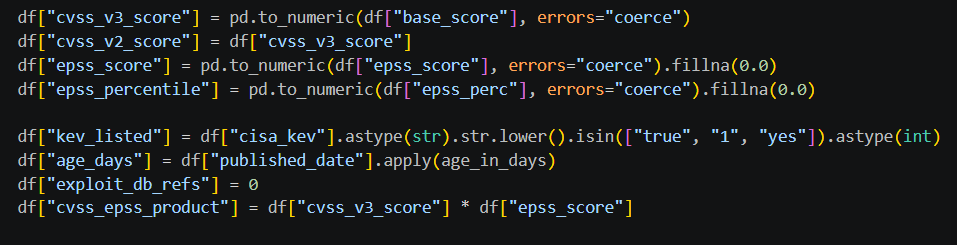
\includegraphics[width=0.9\textwidth]{C-04-AI-Driven Vulnerability Analysis Engine/vertopal_0d07bf200b61446895bb385b0aa02c6b/media/image3.png}
  \caption{Vulnerability-feature engineering implementation of the AVAE.}\label{fig:avae-shap}
\end{figure}

\subsection{Ethics, Privacy, Security, Standards and Responsible AI}\label{sec:method-ethics}

The safety properties of the framework were designed in, not added afterwards.
Four principles govern the deployment of NeuroShell:

\begin{description}
  \item[Sandboxed execution.] Every command runs inside a short-lived,
  locked-down Docker container; the real computer is never exposed. This
  protects against a fixed command harming the host.
  \item[Closed trust boundary.] All model inference runs on the local machine
  through Ollama. No command, error text, or target is transmitted off the
  device, which satisfies strict data-governance requirements of regulated and
  air-gapped environments and addresses the prompt-injection risk of connecting
  an agent to a live network~\cite{liu2023promptinjection}.
  \item[Authorisation and scope enforcement.] The IRE enforces role-based
  authorisation and engagement scope; the AEERE refuses commands that target
  public IP addresses, keeping all work inside RFC-1918 private ranges.
  \item[Test targets are private.] All assessment activity in the project was
  run against private lab addresses that cannot reach any real system, and
  crafted error output is cleaned before it enters an AI prompt to prevent
  prompt-tricking.
\end{description}

The project also follows established standards and frameworks. The development
and evaluation follow the design-science research tradition used across
computer-science theses. For AI governance, the work is aligned with the NIST AI
Risk Management Framework~\cite{nistairmf2023} and, where relevant, with secure
coding guidance such as the OWASP command-injection defence
cheat-sheet~\cite{owasp2025}. Responsible reporting is handled by disclosing the
use of AI assistance during writing and analysis (see
\cref{app:e}). No destructive operation is ever emitted, and every safety
rejection is logged for audit.

\emph{Standards and references shaping the design.} \cref{tab:standards}
records the standards and external references that shaped the design of the
framework, following the same traceability discipline used for the requirements.
The software requirements specification was written against the IEEE 830
recommended practice; the private-address enforcement of both the IRE (S7) and
the AEERE is grounded in RFC 1918; the threat catalogue that motivates the guard
stack follows the OWASP Top 10 for LLM Applications; offline CVE grounding draws
on the National Vulnerability Database as the canonical source of identifiers;
and the tool commands generated at the framework boundary follow the documented
syntax of the respective tools so that contracts are executable by the
downstream components.

\begin{table}[htbp]
  \centering
  \begin{tabular}{@{}p{0.36\textwidth}p{0.56\textwidth}@{}}
    \toprule
    \textbf{Standard or reference} & \textbf{Application in the design}\\
    \midrule
    IEEE 830 recommended practice for SRS & Structure of the requirements specification from which the requirements are derived.\\
    RFC 1918 & Private-address membership tests; restriction of targets to operator-declared private ranges.\\
    OWASP Top 10 for LLM Applications & Threat catalogue that motivates the guard stack.\\
    National Vulnerability Database & Canonical source of CVE identifiers for offline grounding.\\
    Nmap and Metasploit documentation & Syntax of the scanning and exploitation commands suggested in generated contracts.\\
    \bottomrule
  \end{tabular}
  \caption{Standards and references that shaped the NeuroShell design.}\label{tab:standards}
\end{table}

\section{Commercialization Aspects}\label{sec:commercial}

\subsection{Value Proposition and Target Users}\label{sec:commercial-value}

The value proposition of NeuroShell follows from its measured properties rather
than from asserted market figures. For security analysts and operators, the
framework removes manual intent-to-command translation, catches misremembered
syntax, out-of-scope targets, and role violations through deterministic
predicates rather than analyst vigilance, and produces structured responses and
per-request metrics that support audit. For security-tooling integrators, the
IRE exports a closed, schema-enforced contract (nine intent classes, validated
targets, explicit CVE, port, and modifier fields) that replaces prose
re-parsing in orchestrators. For offline-constrained environments, the
framework serves a segment that the surveyed cloud-based copilots do not: it
runs entirely on-device at inference, which is a differentiating fact for
air-gapped, regulated, edge, and research-range deployments.

\subsection{Market and Competitive Position}\label{sec:commercial-market}

The survey of existing systems found four categories (deterministic tooling,
generation-side copilots, tool-integration techniques, and post-hoc
guardrails), each strong in one respect and absent in another. NeuroShell, as a
whole, combines three properties none of the surveyed systems combine:
machine-consumed structured output, schema and scope enforcement, and offline,
CPU-only operation with autonomous error recovery. The AEERE targets the
specific gap left open by PentestGPT, VulnBot, and xOffense: no current AI
security tool fixes its own tool failures on the machine. The gap analysis is
review-based, because no named commercial product was surveyed; no market-share
or revenue claims are made.

\subsection{Business and Sustainability Model}\label{sec:commercial-business}

A business model is described as a set of candidate pathways rather than as
asserted revenue. Because all inference is local and CPU-only, operational
sustainability is low-cost and does not depend on per-call cloud fees. The
planner keeps its documentation store separate from the model, so the knowledge
base can be updated without retraining, which lowers maintenance cost. The
AEERE's error list and tool-swap list can be extended from logged UNKNOWN
errors, giving a data-driven path to keep the engine current as Kali tools
change. Licensing, pricing, and go-to-market details are outside the scope of
this dissertation and are left for a commercialisation plan.

\subsection{Scalability, Intellectual Property and Compliance}\label{sec:commercial-scalability}

The framework was designed to be modular: each component is independently
tested and deployed, which supports scaling out services horizontally. The IRE
and the AEERE run on CPU-only hardware and the AVAE model is small by design,
so the marginal infrastructure cost is low. Compliance-relevant properties
include the closed trust boundary (a strong data-protection argument), the
RFC-1918 scope restriction, and the SQLite audit logs of all safety rejections.
Intellectual-property considerations (patentability, licensing of the model
artefacts, and the documentation knowledge base) are flagged as open
requirements rather than asserted. Verified facts and open requirements are
separated in each component report, and no figure that was not measured is
claimed.

\subsection{Contribution to the Sustainable Development Goals}\label{sec:commercial-sdg}

NeuroShell contributes to several United Nations Sustainable Development Goals.
By automating security workflows and making them safe for less-experienced
operators, it supports building resilient infrastructure (SDG 9). By reducing
the labour and infrastructure cost of security assessment and by running on
shared, low-end hardware, it supports affordable and sustainable industrial
innovation. By protecting data on-premises through a closed trust boundary, it
supports strong institutions and the responsible use of technology. The
component reports map these contributions explicitly; as with all commercial
claims, the mapping is a narrative assessment rather than a measured outcome.

\section{Testing and Implementation}\label{sec:testing}

\subsection{Development Environment and Technology Stack}\label{sec:testing-stack}

All four components were developed in Python and deployed as FastAPI services.
Language-model inference uses Ollama with locally hosted models. The IRE
evaluates two backends (Gemma and Qwen); the planner adapts a Gemma~2 2B
instruction model (exported as a Q8\_0 GGUF artefact and imported into Ollama as
\emph{neuroshell-c2-gemma2-final}); the AEERE uses Gemma through Ollama; the
AVAE uses XGBoost and Scikit-learn. \cref{tab:stack} summarises the common
technology stack.

\begin{table}[htbp]
  \centering
  \begin{tabular}{@{}p{0.36\textwidth}p{0.60\textwidth}@{}}
    \toprule
    \textbf{Layer} & \textbf{Technology used across the framework}\\
    \midrule
    API layer & FastAPI (ports 8001--8004), shared state via Redis\\
    Language models & Gemma 2 2B (Q8\_0 GGUF) and Qwen via Ollama (local only)\\
    Tool documentation & ChromaDB vector store, \emph{all-MiniLM-L6-v2} embeddings\\
    Execution sandbox & Docker containers running Kali Linux\\
    Error-labelling & Hand-written patterns + char n-gram TF-IDF + logistic regression\\
    ML analysis & Pandas, Scikit-learn, XGBoost, SHAP, NumPy\\
    Persistence & SQLite (safety logs), Neo4j (vulnerability graph)\\
    Testing & pytest (unit and integration), pytest-asyncio\\
    \bottomrule
  \end{tabular}
  \caption{Consolidated technology stack of NeuroShell.}\label{tab:stack}
\end{table}

During development, the planner used a Colab environment for GPU-based
adaptation of the Gemma model and Ollama for local deployment; the framework is
intended to operate with local inference only. The model artefact is
approximately 2.8~GB on disk, which is a storage figure and not a minimum
runtime requirement.

\subsection{IRE Implementation, Verification and Testing}\label{sec:testing-ire}

The IRE was implemented as a module-based Python package under fastAPI. The
committed test suite comprises 506 tests (434 unit tests and 72 integration
tests), all of which pass against the current source, with statement coverage of
76\% overall. Coverage is further reported per module against the overall
figure. The evaluation protocol (four experiments, ablation; see
\cref{sec:method-ire}) is executed by a harness that commits per-record
decisions so figures can be audited. Two verified engineering findings were
recorded: a default development API key and an inactive \texttt{production}
scope mode, both flagged as gaps to close before deployment.

\subsection{Planner Implementation, Verification and Testing}\label{sec:testing-planner}

The planner backend was verified with a selected run of the committed test suite
on Windows with Python 3.11.9 and pytest 8.2.0: 42 tests passed with one warning
in 71.28 seconds. The warning concerns a pending deprecation in the \emph{multipart}
import used through Starlette and is not a test failure. The passing cases
support the implemented checks for malformed commands, target and port
contradictions, authentication behaviour, and session recovery. The test areas
and counts are shown in \cref{tab:planner-tests}.

\begin{table}[htbp]
  \centering
  \begin{tabular}{@{}p{0.50\textwidth}p{0.20\textwidth}@{}}
    \toprule
    \textbf{Test area} & \textbf{Passed tests}\\
    \midrule
    Planning API integration & 14\\
    Command validator & 3\\
    Safety filter & 4\\
    Intent interpreter & 6\\
    Command evaluator & 15\\
    \midrule
    Total & 42\\
    \bottomrule
  \end{tabular}
  \caption{Selected software verification results of the planner.}\label{tab:planner-tests}
\end{table}

\subsection{AEERE Implementation, Verification and Testing}\label{sec:testing-aeere}

The error-labelling test (SO3) was measured and is reported in
\cref{ch:results}: the three-step cascade reaches a macro-F1 of 100\% on the
clean data set and 99.1\% at 30\% message noise, remaining above 96\% even at
60\% noise. The pattern step runs in about 0.004~ms per message and the text
model in about 0.5~ms. The remaining verification targets (the overall fix rate,
the end-to-end speed and cost of a full fix, and the dangerous-command block
rate) require the full engine running on real hardware with Docker and Ollama,
which was not available at the time the component report was written. Those
tables are therefore recorded for the live engine; no result is invented. The
reported measurements are the labelling performance and per-step latency only.

\subsection{AVAE Implementation, Verification and Testing}\label{sec:testing-avae}

\begin{sloppypar}
Verification of the AVAE focuses on input processing, scanner-output parsing,
vulnerability-intelligence enrichment, machine-learning prediction, SHAP
explanation generation, API response handling, and graph persistence. Machine
learning verification evaluates the XGBoost classifier with the standard
classification metrics; software testing verifies that supported inputs are
processed correctly, relevant findings are extracted, and structured responses
are generated. The provisional model results are reported in \cref{ch:results}
with the explicit caveat, stated in the component report, that the final
conclusions require the confirmed, verified evaluation results.
\end{sloppypar}

\subsection{Integration Testing}\label{sec:testing-integration}

Integration testing verifies the hand-over between components. Selected API
tests passed for the planner's input handling, authentication, rejection, and
session-dependent target recovery. Local inference demonstrated an explicit Nmap
port request that produced \texttt{nmap -p 22,80,443 192.168.1.10} in both the
Colab adapter check and the Ollama check, and a service-detection request
produced \texttt{nmap -sV 192.168.50.10} locally. These are individual
generation checks rather than aggregate integration-accuracy measures. The AVAE
integration workflow verifies C3--C4 communication (structured execution-result
transfer), output parsing, ML prediction, SHAP explainability, Neo4j
integration, and API response generation. The complete integration outcome
across all four components requires confirmation through recorded end-to-end
testing evidence, which no single component report collects on its own.

\subsection{Deployment and Operation}\label{sec:testing-deploy}

Each component deploys as an independent FastAPI service. The IRE and the AEERE
use Ollama for local model inference (no cloud dependency). The planner imports
its adapted model as \emph{neuroshell-c2-gemma2-final} in Ollama and retains
ChromaDB as a persistent knowledge base. The AEERE requires Docker and Redis;
its \texttt{/execute} endpoint accepts a \texttt{PlannerOutput} and returns an
\texttt{ExecutionResult} with a status of \texttt{success}, \texttt{recovered},
or \texttt{failed}, a fix log, and a failure report, with a \texttt{/health}
check reporting whether the service and Docker are up. The AVAE loads its ML
artefacts at startup and exposes \texttt{/analyze} to receive structured
execution results and return analysis outputs. Because inference is local and
CPU-based, the framework can be operated on a single machine, which also
simplifies the operational sustainability model described in
\cref{sec:commercial-business}.